%%%%%%%%%%%%%%%%%%%%%%%%%%%%%%%%%%%%%%%%%%%%%%%%%%%%%%%%%%%%%%%%%%
%%%%%%%%%%%%%%%%%%%%%%%%%%%%%%%%%%%%%%%%%%%%%%%%%%%%%%%%%%%%%%%%%%
%Packages
\documentclass[10pt, a4paper]{article}
\usepackage[top=3cm, bottom=4cm, left=3.5cm, right=3.5cm]{geometry}
\usepackage{amsmath,amsthm,amsfonts,amssymb,amscd, fancyhdr, color, comment, graphicx, environ}
\usepackage{float}
\usepackage{mathrsfs}
\usepackage[math-style=ISO]{unicode-math}
\setmathfont{TeX Gyre Termes Math}
\usepackage{lastpage}
\usepackage[dvipsnames]{xcolor}
\usepackage[framemethod=TikZ]{mdframed}
\usepackage{enumerate}
\usepackage[shortlabels]{enumitem}
\usepackage{fancyhdr}
\usepackage{indentfirst}
\usepackage{listings}
\usepackage{sectsty}
\usepackage{thmtools}
\usepackage{shadethm}
\usepackage{hyperref}
\usepackage{setspace}
\hypersetup{
    colorlinks=true,
    linkcolor=blue,
    filecolor=magenta,      
    urlcolor=blue,
}
\usepackage[makeroom]{cancel}
\usepackage[utf8]{inputenc}
\usepackage[T1]{fontenc}
\usepackage{hyperref}
\hypersetup{colorlinks=true, linkcolor=blue, filecolor=magenta, urlcolor=cyan,}
\urlstyle{same}
\usepackage{amsmath}
\usepackage{amsfonts}
\usepackage{amssymb}
\usepackage[version=4]{mhchem}
\usepackage{stmaryrd}
\usepackage{graphicx}
\usepackage[export]{adjustbox}
\graphicspath{ {./images/} }
\usepackage{listings}
%%%%%%%%%%%%%%%%%%%%%%%%%%%%%%%%%%%%%%%%%%%%%%%%%%%%%%%%%%%%%%%%%%
%%%%%%%%%%%%%%%%%%%%%%%%%%%%%%%%%%%%%%%%%%%%%%%%%%%%%%%%%%%%%%%%%%
%Environment setup
\mdfsetup{skipabove=\topskip,skipbelow=\topskip}
\newrobustcmd\ExampleText{%
An \textit{inhomogeneous linear} differential equation has the form
\begin{align}
L[v ] = f,
\end{align}
where $L$ is a linear differential operator, $v$ is the dependent
variable, and $f$ is a given non−zero function of the independent
variables alone.
}
\mdfdefinestyle{theoremstyle}{%
linecolor=black,linewidth=1pt,%
frametitlerule=true,%
frametitlebackgroundcolor=gray!20,
innertopmargin=\topskip,
}
\mdtheorem[style=theoremstyle]{Problem}{Problem}
\newenvironment{Solution}{\textbf{Solution.}}

\definecolor{codegreen}{rgb}{0,0.6,0}
\definecolor{codegray}{rgb}{0.5,0.5,0.5}
\definecolor{codepurple}{rgb}{0.58,0,0.82}
\definecolor{backcolour}{rgb}{0.95,0.95,0.92}

\lstdefinestyle{mystyle}{
    backgroundcolor=\color{backcolour},   
    commentstyle=\color{codegreen},
    keywordstyle=\color{magenta},
    numberstyle=\tiny\color{codegray},
    stringstyle=\color{codepurple},
    basicstyle=\ttfamily\footnotesize,
    breakatwhitespace=false,         
    breaklines=true,                 
    captionpos=b,                    
    keepspaces=true,                 
    numbers=left,                    
    numbersep=5pt,                  
    showspaces=false,                
    showstringspaces=false,
    showtabs=false,                  
    tabsize=2
}

\lstset{style=mystyle}
%%%%%%%%%%%%%%%%%%%%%%%%%%%%%%%%%%%%%%%%%%%%%%%%%%%%%%%%%%%%%%%%%%
%%%%%%%%%%%%%%%%%%%%%%%%%%%%%%%%%%%%%%%%%%%%%%%%%%%%%%%%%%%%%%%%%%
%Fill in the appropriate information below
\newcommand{\norm}[1]{\left\lVert#1\right\rVert}     
\newcommand\course{CS5785}                            % <-- course name   
\newcommand\hwnumber{2}                                 % <-- homework number
\newcommand\Information{Arystan Tatishev, Maanas Peri}                        % <-- personal information
%%%%%%%%%%%%%%%%%%%%%%%%%%%%%%%%%%%%%%%%%%%%%%%%%%%%%%%%%%%%%%%%%%
%%%%%%%%%%%%%%%%%%%%%%%%%%%%%%%%%%%%%%%%%%%%%%%%%%%%%%%%%%%%%%%%%%
%Page setup
\pagestyle{fancy}
\headheight 35pt
\lhead{\today}
\rhead{
\includegraphics[width=2.5cm]{logo-ct.png}}
\lfoot{}
\pagenumbering{arabic}
\cfoot{\small\thepage}
\rfoot{}
\headsep 1.2em
\renewcommand{\baselinestretch}{1.25}
%%%%%%%%%%%%%%%%%%%%%%%%%%%%%%%%%%%%%%%%%%%%%%%%%%%%%%%%%%%%%%%%%%
%%%%%%%%%%%%%%%%%%%%%%%%%%%%%%%%%%%%%%%%%%%%%%%%%%%%%%%%%%%%%%%%%%
%Add new commands here
\renewcommand{\labelenumi}{\alph{enumi})}
\newcommand{\Z}{\mathbb Z}
\newcommand{\R}{\mathbb R}
\newcommand{\Q}{\mathbb Q}
\newcommand{\NN}{\mathbb N}
\newcommand{\PP}{\mathbb P}
\DeclareMathOperator{\Mod}{Mod} 
\renewcommand\lstlistingname{Algorithm}
\renewcommand\lstlistlistingname{Algorithms}
\def\lstlistingautorefname{Alg.}
\newtheorem*{theorem}{Theorem}
\newtheorem*{lemma}{Lemma}
\newtheorem{case}{Case}
\newcommand{\assign}{:=}
\newcommand{\infixiff}{\text{ iff }}
\newcommand{\nobracket}{}
\newcommand{\backassign}{=:}
\newcommand{\tmmathbf}[1]{\ensuremath{\boldsymbol{#1}}}
\newcommand{\tmop}[1]{\ensuremath{\operatorname{#1}}}
\newcommand{\tmtextbf}[1]{\text{{\bfseries{#1}}}}
\newcommand{\tmtextit}[1]{\text{{\itshape{#1}}}}

\newenvironment{itemizedot}{\begin{itemize} \renewcommand{\labelitemi}{$\bullet$}\renewcommand{\labelitemii}{$\bullet$}\renewcommand{\labelitemiii}{$\bullet$}\renewcommand{\labelitemiv}{$\bullet$}}{\end{itemize}}
\catcode`\<=\active \def<{
\fontencoding{T1}\selectfont\symbol{60}\fontencoding{\encodingdefault}}
\catcode`\>=\active \def>{
\fontencoding{T1}\selectfont\symbol{62}\fontencoding{\encodingdefault}}
\catcode`\<=\active \def<{
\fontencoding{T1}\selectfont\symbol{60}\fontencoding{\encodingdefault}}

%%%%%%%%%%%%%%%%%%%%%%%%%%%%%%%%%%%%%%%%%%%%%%%%%%%%%%%%%%%%%%%%%%
%%%%%%%%%%%%%%%%%%%%%%%%%%%%%%%%%%%%%%%%%%%%%%%%%%%%%%%%%%%%%%%%%%
%Begin now!



\begin{document}

\begin{titlepage}
    \begin{center}
        \vspace*{3cm}
            
        \Huge
        \textbf{Assignment}
            
        \vspace{1cm}
        \huge
        Homework \hwnumber
            
        \vspace{1.5cm}
        \Large
            
        \textbf{\Information}                      % <-- author
        
            
        \vfill
        
        A \course \ Homework Assignment
            
        \vspace{1cm}
            
        
\includegraphics[width=0.4\textwidth]{logo-ct.png}
        \\
        
        \Large
        
        \today
            
    \end{center}
\end{titlepage}

%%%%%%%%%%%%%%%%%%%%%%%%%%%%%%%%%%%%%%%%%%%%%%%%%%%%%%%%%%%%%%%%%%
%%%%%%%%%%%%%%%%%%%%%%%%%%%%%%%%%%%%%%%%%%%%%%%%%%%%%%%%%%%%%%%%%%
%Start the assignment now
%%%%%%%%%%%%%%%%%%%%%%%%%%%%%%%%%%%%%%%%%%%%%%%%%%%%%%%%%%%%%%%%%%
%New problem
\newpage
\section*{Programming Exercises}
\section*{Binary Classification on Text Data}
\begin{Problem}
In this problem, you will implement several machine learning techniques from the class to perform classification on text data. Throughout the problem, we will be working on the NLP with Disaster Tweets Kaggle competition, where the task is to predict whether or not a tweet is about a real disaster.
\end{Problem}

\begin{Problem*}[(a) Download the data. ]
    Download the training and test data from Kaggle, and answer the following questions: (1) how many training and test data points are there? and (2) what percentage of the training tweets are of real disasters, and what percentage is not? Note that the meaning of each column is explained in the data description on Kaggle.
\end{Problem*}

\begin{Solution}
\begin{lstlisting}[language=Python]
from google.colab import drive
drive.mount("/content/gdrive")

import nltk
nltk.download('all')

import pandas as pd

training_data = pd.read_csv("/content/sample_data/train.csv")
testing_data = pd.read_csv("/content/sample_data/test.csv")

percentTrue = training_data['target'].value_counts()[1]
percentFalse = training_data['target'].value_counts()[0]
print("Percentage of the training tweets that are of real disasters is %", (percentTrue/len(training_data['target'])) * 100)
print("Percentage of the training tweets that are not of real disasters is %", (percentFalse/len(training_data['target'])) * 100)

print(training_data.describe())
print("\n", training_data.head())

print("here: ", training_data["text"][4])
print("here: ", testing_data["text"][4])

Y_training = training["target"]
X_training = training.drop("target", axis = 1)

Y_test = testing["target"]
X_test = testing.drop("target", axis = 1)

percent_missing_train = X_training.isnull().sum() * 100 / len(X_training)
total_missing_train = X_training.isnull().sum()
print("percent missing in X_train: ", percent_missing_train)
'''
percent missing in X_train:  id           0.000000
keyword      0.825671
location    33.627322
text         0.000000

Going to drop location and keyword
'''
print("total missing in X_train: ", total_missing_train)
'''
total missing in X_train:  id             0
keyword       44
location    1792
text           0
dtype: int64
'''
X_training = X_training.drop("location", axis=1)
X_training = X_training.drop("keyword", axis=1)
X_training = X_training.drop("id", axis=1)

X_test = X_test.drop("location", axis=1)
X_test = X_test.drop("keyword", axis=1)
X_test = X_test.drop("id", axis=1)

print(X_test.head())
print(X_test.describe())

print(X_training.shape)
print(X_test.shape)
\end{lstlisting}

\begin{figure}
    \centering
    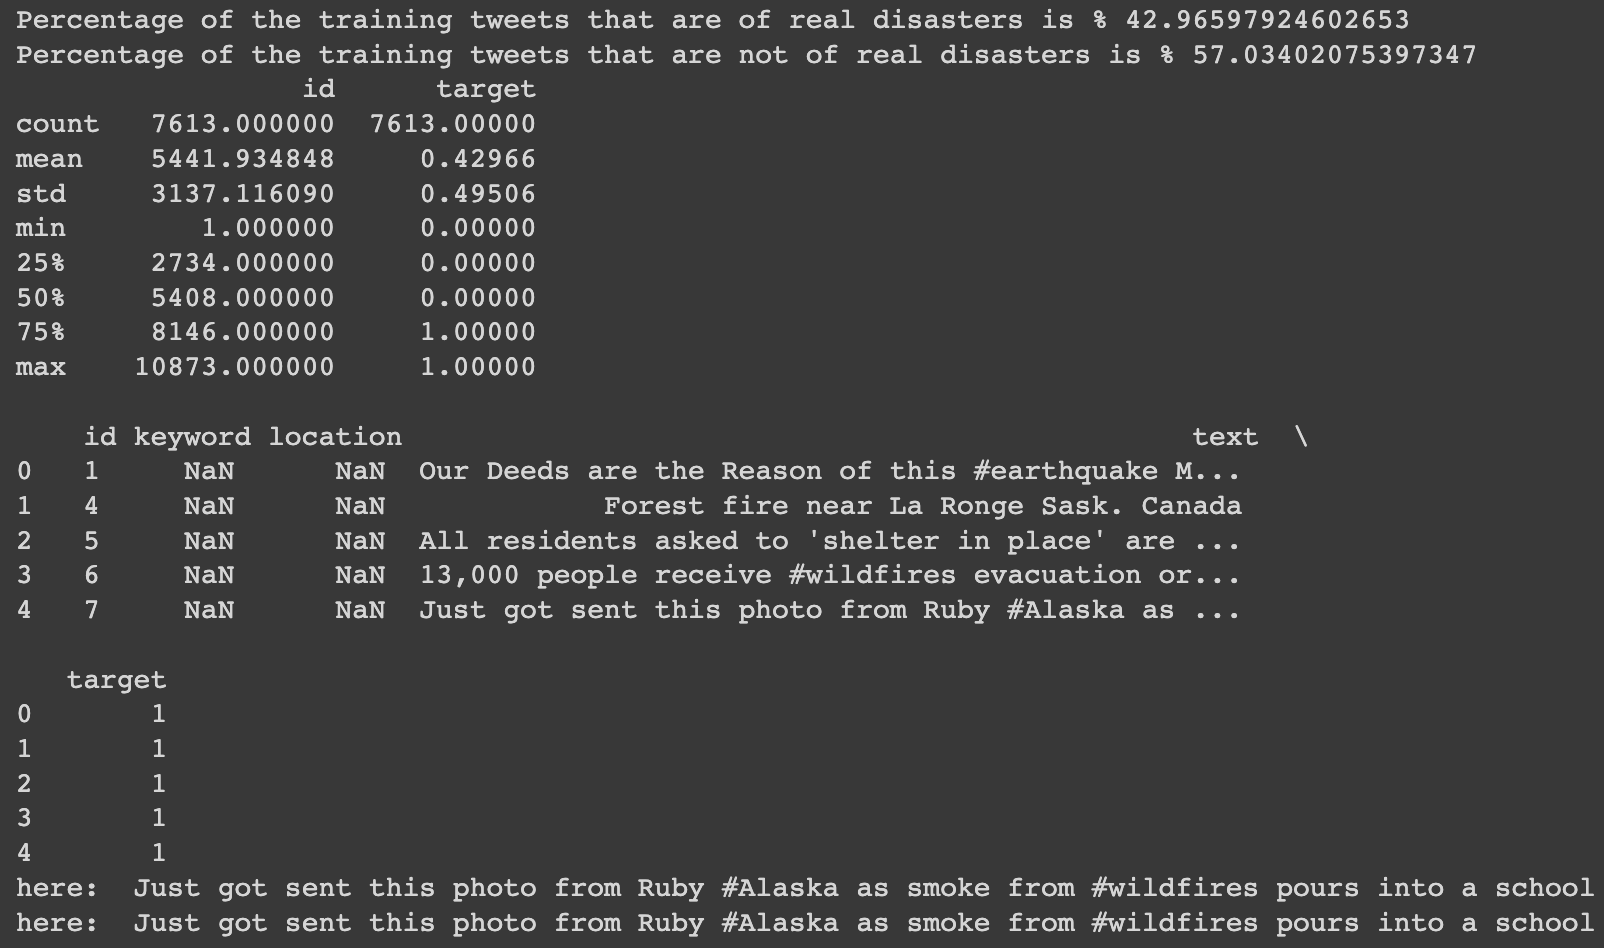
\includegraphics[width=0.75\linewidth]{HW2//images/img1.png}
\end{figure}

\end{Solution}

\begin{Problem*}[(b) Split the training data. ]
    Since we do not know the correct values of labels in the test data, we will split the training data from Kaggle into a training set and a development set (a development set is a held out subset of the labeled data that we set aside in order to fine-tune models, before evaluating the best model(s) on the test data). Randomly choose $70 \%$ of the data points in the training data as the training set, and the remaining $30 \%$ of the data as the development set. Throughout the rest of this problem we will keep these two sets fixed. The idea is that we will train different models on the training set, and compare their performance on the development set, in order to decide what to submit to Kaggle.
\end{Problem*}

\begin{Solution}
\begin{lstlisting}[language=Python]
import random

# 70% training data, 30% evaluation data
shuffledData = training_data.sample(frac = 1)
training = shuffledData[:int(len(shuffledData) * 0.70)]
testing = shuffledData[int(len(shuffledData) * 0.70):]

Y_training = training["target"]
X_training = training.drop("target", axis = 1)

Y_test = testing["target"]
X_test = testing.drop("target", axis = 1)

percent_missing_train = X_training.isnull().sum() * 100 / len(X_training)
total_missing_train = X_training.isnull().sum()
print("percent missing in X_train: ", percent_missing_train)
'''
percent missing in X_train:  id           0.000000
keyword      0.825671
location    33.627322
text         0.000000

Going to drop location and keyword
'''
print("total missing in X_train: ", total_missing_train)
'''
total missing in X_train:  id             0
keyword       44
location    1792
text           0
dtype: int64
'''

X_training = X_training.drop("location", axis=1)
X_training = X_training.drop("keyword", axis=1)
X_training = X_training.drop("id", axis=1)

X_test = X_test.drop("location", axis=1)
X_test = X_test.drop("keyword", axis=1)
X_test = X_test.drop("id", axis=1)

\end{lstlisting}


\end{Solution}

\begin{Problem*}[(c) Preprocess the data. ]
    Since the data consists of tweets, they may contain significant amounts of noise and unprocessed content. You may or may not want to do one or all of the following. Explain the reasons for each of your decision (why or why not).

\begin{itemize}
  \item Convert all the words to lowercase.

  \item Lemmatize all the words (i.e., convert every word to its root so that all of "running," "run," and "runs" are converted to "run" and and all of "good," "well," "better," and "best" are converted to "good"; this is easily done using nltk.stem).

  \item Strip punctuation.

  \item Strip the stop words, e.g., "the”, "and”, “or”.

  \item Strip @ and urls. (It’s Twitter.)

  \item Something else? Tell us about it.

\end{itemize}
\end{Problem*}

\begin{Solution}
\begin{lstlisting}[language=Python]
pd.options.mode.chained_assignment = None  # Suppress the warning
X_training.loc[:,"text"] = X_training["text"].str.lower()
print(X_training["text"].head())
print(X_test["text"].head())

stopwording = nltk.corpus.stopwords.words("english")
#we need to tokenize each word in the sentence and then
def lemmatize_text(line):
    #tokenizing, and then
    listOfWords = nltk.word_tokenize(line)
    listOfWords = [word for word in listOfWords if word.isalnum()]
    listOfWords = [word for word in listOfWords if word not in stopwording]

    lemmatized = []
    for word in listOfWords:
        lemWord = nltk.stem.wordnet.WordNetLemmatizer().lemmatize(word)
#         print(lemWord)
        lemmatized.append(lemWord)
    return ' '.join(lemmatized) #we want to return a line of stemmed words, not a array bc it has to be replaced in the pandas dataframe

# text = "our deeds are the reason of this #earthquake may allah forgive us all"

X_training["text"] = X_training["text"].apply(lemmatize_text) #applying this function for every line
X_test["text"] = X_test["text"].apply(lemmatize_text) #applying this function for every line

print("Training After: ", X_training["text"])
print("Testing After: ", X_test["text"])
\end{lstlisting}


\end{Solution}

\begin{Problem*}[(d) Bag of words model.]
     The next task is to extract features in order to represent each tweet using the binary "bag of words" model, as discussed in lectures. The idea is to build a vocabulary of the words appearing in the dataset, and then to represent each tweet by a feature vector $x$ whose length is the same as the size of the vocabulary, where $x_{i}=1$ if the $i$ 'th vocabulary word appears in that tweet, and $x_{i}=0$ otherwise. In order to build the vocabulary, you should choose some threshold $M$, and only include words that appear in at least $k$ different tweets; this is important both to avoid run-time and memory issues, and to avoid noisy/unreliable features that can hurt learning. Decide on an appropriate threshold $M$, and discuss how you made this decision. Then, build the bag of words feature vectors for both the training and development sets, and report the total number of features in these vectors.

In order to construct these features, we suggest using the CountVectorizer class in sklearn. A couple of notes on using this function: (1) you should set the option "binary=True" in order to ensure that the feature vectors are binary; and (2) you can use the option "min\_df=M" in order to only include in the vocabulary words that appear in at least $M$ different tweets. Finally, make sure you fit CountVectorizer only once on your training set and use the same instance to process both your training and development sets (don't refit it on your development set a second time).

Important: at this point you should only be constructing feature vectors for each data point using the text in the "text" column. You should ignore the "keyword" and "location" columns for now.
\end{Problem*}

\begin{Solution}
\begin{lstlisting}[language=Python]
from sklearn.feature_extraction.text import CountVectorizer

M = 2
bow_vectorizer = CountVectorizer(binary = True, min_df = M)

X_trainBOW = bow_vectorizer.fit_transform(X_training["text"]).toarray()
X_testBOW = bow_vectorizer.transform(X_test["text"]).toarray()

#feature size of training and testing matrices
print("Training data shape before:", X_trainBOW.shape)
print("Testing data shape before:", X_testBOW.shape)
\end{lstlisting}
\end{Solution}

\begin{Problem*}[(e) Logistic regression. ]
    In this question, we will be training logistic regression models using bag of words feature vectors obtained in part (d). We will use the $F 1$-score as the evaluation metric.

Note that the $F 1$-score, also known as $F$-score, is the harmonic mean of precision and recall. Recall that precision and recall are:

$$
\text { precision }=\frac{\# \text { true positives }}{\# \text { true positives }+\# \text { false positives }} \quad 
$$

$$
\text { recall }=\frac{\# \text { true positives }}{\# \text { true positives }+\# \text { false negatives }} \text {. }
$$

$F 1$-score is the harmonic mean (or, see it as a weighted average) of precision and recall:

$$
F 1=\frac{2}{\text { precision }^{-1}+\text { recall }^{-1}}=2 \frac{\text { precision } \cdot \text { recall }}{\text { precision }+ \text { recall }}
$$

We use $F 1$-score because it gives a more comprehensive view of classifier performance than accuracy. For more information on this metric see F1-score.

We ask you to train the following classifiers. We suggest using the LogisticRegression implementation in sklearn.
\end{Problem*}

\begin{Problem*}[i.]
    Train a logistic regression model without regularization terms. You will notice that the default sklearn logistic regression utilizes L2 regularization. You can turn off L2 regularization by changing the penalty parameter. Report the F1 score in your training and in your development set. Comment on whether you observe any issues with overfitting or underfitting.
\end{Problem*}

\begin{Solution}
\begin{lstlisting}[language=Python]
from sklearn.linear_model import LogisticRegression
from sklearn.metrics import f1_score

logic_reg = LogisticRegression(penalty='none', verbose = True)
logic_reg.fit(X_trainBOW, Y_training)
predY_train_LR = logic_reg.predict(X_trainBOW)
predY_test_LR = logic_reg.predict(X_testBOW)

print(X_trainBOW.shape, predY_train_LR.shape)

train_f1 = f1_score(Y_training, predY_train_LR)
dev_f1 = f1_score(Y_test, predY_test_LR)

print("F1 Score on Training Set (without regularization):", train_f1)
print("F1 Score on Development Set (without regularization):", dev_f1)
\end{lstlisting}

F1 Score on Training Set (without regularization): 0.9818022363516772
F1 Score on Development Set (without regularization): 0.7001491795126802

\end{Solution}

\begin{Problem*}[ii.]
    Train a logistic regression model with $\mathrm{L} 1$ regularization. Sklearn provides some good examples for implementation. Report the performance on both the training and the development sets.
\end{Problem*}

\begin{Solution}
\begin{lstlisting}[language=Python]
from sklearn.linear_model import LogisticRegression
from sklearn.metrics import f1_score

logic_reg_L1 = LogisticRegression(penalty='l1', verbose = True, solver='liblinear')
logic_reg_L1.fit(X_trainBOW, Y_training)

predY_train_L1 = logic_reg_L1.predict(X_trainBOW)
predY_test_L1 = logic_reg_L1.predict(X_testBOW)

print(X_trainBOW.shape, predY_train_L1.shape)

train_f1_L1 = f1_score(Y_training, predY_train_L1)
dev_f1_L1 = f1_score(Y_test, predY_test_L1)


print("F1 Score on Training Set (with L1 regularization):", train_f1_L1)
print("F1 Score on Development Set (with L1 regularization):", dev_f1_L1)
\end{lstlisting}

F1 Score on Training Set (with L1 regularization): 0.8546578164339667
F1 Score on Development Set (with L1 regularization): 0.7176602924634421
\end{Solution}

\begin{Problem*}[iii.]
    Similarly, train a logistic regression model with L2 regularization. Report the performance on the training and the development sets.
\end{Problem*}

\begin{Solution}
\begin{lstlisting}[language=Python]
from sklearn.linear_model import LogisticRegression
from sklearn.metrics import f1_score

logic_reg = LogisticRegression(penalty='l2', verbose = True, solver='liblinear')
logic_reg.fit(X_trainBOW, Y_training)

predY_train_L2 = logic_reg.predict(X_trainBOW)
predY_test_L2 = logic_reg.predict(X_testBOW)

print(X_trainBOW.shape, predY_train_L2.shape)

train_f1_L2 = f1_score(Y_training, predY_train_L2)
dev_f1_L2 = f1_score(Y_test, predY_test_L2)


print("F1 Score on Training Set (with L2 regularization):", train_f1_L2)
print("F1 Score on Development Set (with L2 regularization):", dev_f1_L2)
\end{lstlisting}

F1 Score on Training Set (with L2 regularization): 0.9118843199277
F1 Score on Development Set (with L2 regularization): 0.7280848687883864

\end{Solution}

\begin{Problem*}[iv.]
    Which one of the three classifiers performed the best on your training and development set? Did you observe any overfitting and did regularization help reduce it? Support your answers with the classifier performance you got.
\end{Problem*}

\begin{Solution}
The best performing classifier was L2 regularization. Yes, there was overfitting for the unregularized classifier with the F score being 0.98 on the training set. So after the L2 regularization the F score for the training set dropped to 0.91 but the development set F score improved from 0.70 to 0.74


\end{Solution}

\begin{Problem*}[v.]
    Inspect the weight vector of the classifier with L1 regularization (in other words, look at the $\theta$ you got after training). You can access the weight vector of the trained model using the coef\_attribute of a LogisticRegression instance. What are the most important words for deciding whether a tweet is about a real disaster or not?
\end{Problem*}

\begin{Solution}
\begin{lstlisting}[language=Python]
import numpy as np

coeff = logic_reg_L1.coef_[0]
# print(coeff)

feature_names = bow_vectorizer.get_feature_names_out()
# print(feature_names)

word_coefficients = dict(zip(feature_names, coeff))
sorted_word_coefficients = sorted(word_coefficients.items(), key=lambda x: abs(x[1]), reverse=True)

#top 10
for word, coefficient in sorted_word_coefficients[:10]:
    print(f"Word: {word}, Coefficient: {coefficient}")
\end{lstlisting}

Word: hiroshima, Coefficient: 2.3554390536812364
Word: earthquake, Coefficient: 2.311429233550751
Word: wildfire, Coefficient: 2.0151127646081
Word: typhoon, Coefficient: 1.8830269877431178
Word: derailment, Coefficient: 1.8675710454576782
Word: train, Coefficient: 1.8495430330025884
Word: storm, Coefficient: 1.7660768891744731
Word: japan, Coefficient: 1.7226607378999386
Word: tornado, Coefficient: 1.714069245568201
Word: flood, Coefficient: 1.7102663944043897
\end{Solution}

\begin{Problem*}[(f) Bernoulli Naive Bayes]
    Implement a Bernoulli Naive Bayes classifier to predict the probability of whether each tweet is about a real disaster. Train this classifier on the training set, and report its $F 1$-score on the development set.

Important: For this question you should implement the classifier yourself similar to what was shown in class, without using any existing machine learning libraries such as sklearn. You may only use basic libraries such as numpy.

As you work on this problem, you may find that there exists some words that only appear in some classes but never in other classes in the training set. This might lead the model into thinking it is impossible for the word to appear in those other classes it never appears in in the training set, even though that word might actually appear in those classes in the development set.

Concretely, suppose word $j$ never appears in class $k$ in the training set. Since the maximum likelihood estimate of $\psi_{j k}$ is $\frac{n_{j k}}{n_{k}}$ where $n_{k}$ is the number of documents of class $k$ and $n_{j k}$ is the number of documents of class $k$ that contain word $j$, during training, we set

$$
P\left(x_{j}=1 \mid y=k\right)=\psi_{j k}=\frac{n_{j k}}{n_{k}}=0
$$

Then, any bag of words $x$ that contains word $j$, i.e., $x_{j}=1$, will have

$$
P_{\theta}(x \mid y=k)=\prod_{j=1}^{d} P\left(x_{j} \mid y=k\right)=0
$$

We obviously do not want this, because this implies we only assign positive probability to the bag of words whose words have appeared in the class $k$ at least once.

The solution to this problem is a form of regularization called Laplace smoothing or additive smoothing. The idea is to use "pseudo-counts", i.e. to increment the number of times we have seen class $k$ document with word $j$ by some number of "virtual" occurrences $\alpha$, and increment the number of times we have seen class $k$ document in general by $2 \alpha$ (so half of the pseudo documents have word $j$ in it). Mathematically,

$$
\psi_{j k}=\frac{n_{j k}+\alpha}{n_{k}+2 \alpha}
$$

Thus, the Naive Bayes model will behave as if every word or document has been seen at least $\alpha$ times.

It's normal to take $\alpha=1$.
\end{Problem*}

\begin{Solution}
\begin{lstlisting}[language=Python]
class BernoulliNB:
    def __init__(self, alpha=1):
        self.alpha = alpha

    def training(self, BOW_X_train, Y_train):
        unique_classes = np.unique(Y_train)

        # initialization for Laplace smoothing in predict function
        self.classes = {}
        for c in unique_classes:
            self.classes[c] = np.ones(BOW_X_train.shape[1]) * self.alpha #calculating the proportion of training samples that belong to class c

        self.word_counts = {}
        for c in unique_classes:
            #still needs fixing
            self.word_counts[c] = np.ones(BOW_X_train.shape[1]) * self.alpha

        self.class_counts = {}
        for c in unique_classes:
            self.class_counts[c] = np.ones(BOW_X_train.shape[1]) * self.alpha

        # where the real counting begins. Dictionaries created, and then manipulated where we have our Y_training data
        for c in unique_classes:
            X_c = BOW_X_train[Y_train == c] #filtering where the unique classes exist in Y_training, that way we can match with X-training that is relevant. Need to train on this filtered data
            self.word_counts[c] += X_c.sum(axis=0)
            self.class_counts[c] += len(X_c)
            self.classes[c] = np.mean(Y_train == c)

    #used gpt to aid with building the predict function and debugging
    def predict(self, BOW_X_dev):
        num_samples = BOW_X_dev.shape[0]  # Number of samples in X_dev
        num_classes = len(self.classes)
        predictions = []

        for i in range(num_samples):
            sample = BOW_X_dev[i]
            class_scores = {}

            for c in self.classes:
                # Calculate log-likelihood for class c, Laplace Smoothing taking place
                log_likelihood = np.sum(
                    np.log((self.word_counts[c] + self.alpha) / (self.class_counts[c] + 2 * self.alpha)) * sample +
                    np.log(1 - (self.word_counts[c] + self.alpha) / (self.class_counts[c] + 2 * self.alpha)) * (1 - sample)
                )

                # Calculate log posterior for class c
                log_posterior = np.log(self.class_priors[c]) + log_likelihood
                class_scores[c] = log_posterior

            # Predict the class with the highest log posterior
            predicted_class = max(class_scores, key=class_scores.get)
            predictions.append(predicted_class)

        return predictions

nb = BernoulliNB(alpha=1)
nb.training(X_trainBOW, Y_training)
predY_train_Bnb = nb.predict(X_trainBOW)
predY_test_Bnb = nb.predict(X_testBOW)

train_f1_Bnb = f1_score(Y_training, predY_train_Bnb)
dev_f1_Bnb = f1_score(Y_test, predY_test_Bnb)

print("F1 Score on Training Set (Bernoulli Naive Bayes):", train_f1_Bnb)
print("F1 Score on Development Set (Bernoulli Naive Bayes):", dev_f1_Bnb)
\end{lstlisting}

F1 Score on Training Set (Bernoulli Naive Bayes): 0.8212608158220024
F1 Score on Development Set (Bernoulli Naive Bayes): 0.7107728337236534

\end{Solution}

\begin{Problem*}[(g) Model comparison.]
     You just implemented a generative classifier and a discriminative classifier. Reflect on the following:

\begin{itemize}
  \item Which model performed the best in predicting whether a tweet is of a real disaster or not? Include your performance metric in your response. Comment on the pros and cons of using generative vs discriminative models.

  \item Think about the assumptions that Naive Bayes makes. How are the assumptions different from logistic regressions? Discuss whether it's valid and efficient to use Bernoulli Naive Bayes classifier for natural language texts.
\end{itemize}
\end{Problem*}

\begin{Solution}
*   Which model performed the best in predicting whether a tweet is of a real disaster or not?

The generative model achieved an F1 score of 0.725, while the L2 discriminative model achieved an F1 score of 0.741. Therefore, the discriminative model performed better in predicting whether a tweet is of a real disaster or not.

The pros of using generative models are that they can handle missing data and can generate new data. The cons are that they can be prone to overfitting the data.

The pros of using discriminative models are that they can be simpler and faster than generative models, and they can perform well in classification tasks. The cons are that they may not handle missing data well and may not be able to generate new data.


*   Think about the assumptions that Naive Bayes makes. How are the assumptions different from logistic regressions?

The assumptions that Naive Bayes makes are that the features are conditionally independent given the class, and that the distribution of the features is known. Logistic regression does not make these assumptions. It assumes that the relationship between the features and the class is linear.

\end{Solution}

\begin{Problem*}[(h) N-gram model.]
    The $\mathrm{N}$-gram model is similar to the bag of words model, but instead of using individual words we use $\mathrm{N}$-grams, which are contiguous sequences of words. For example, using $N=2$, we would says that the text "Alice fell down the rabbit hole" consists of the sequence of 2-grams: ["Alice fell", "fell down", "down the", "the rabbit", "rabbit hole"], and the following sequence of 1-grams: ["Alice", "fell", "down", "the", "rabbit", "hole"]. All eleven of these symbols may be included in the vocabulary, and the feature vector $x$ is defined according to $x_{i}=1$ if the $i$ 'th vocabulary symbol occurs in the tweet, and $x_{i}=0$ otherwise. Using $N=2$, construct feature representations of the tweets in the training and development tweets. Again, you should choose a threshold $M$, and only include symbols in the vocabulary that occur in at least $M$ different tweets in the training set. Discuss how you chose the threshold $M$, and report the total number of 2-grams in your vocabulary. In addition, take 10 2-grams from your vocabulary, and print them out.

    Then, implement a logistic regression and a Bernoulli classifier to train on 2-grams. You may reuse the code in (e) and (f). You may also choose to use or not use a regularization term, depending on what you got from (e). Report your results on training and development set. Do these results differ significantly from those using the bag of words model? Discuss what this implies about the task.

Again, we suggest using CountVectorizer to construct these features. To get 2-grams, you can set ngram\_range $=(2,2)$ for CountVectorizer. Note also that in this case, since there are probably many different 2 -grams in the dataset, it is especially important carefully set min\_df in order to avoid run-time and memory issues.
\end{Problem*}

\begin{Solution}
\begin{lstlisting}[language=Python]
M = 2
n_gram_vectorizer = CountVectorizer(binary = True, min_df = M, ngram_range=(1,2))

X_train_NGram = n_gram_vectorizer.fit_transform(X_training["text"]).toarray()
X_test_NGram = n_gram_vectorizer.transform(X_test["text"]).toarray()

#feature size of training and testing matrices
print("Training data shape before:", X_train_NGram.shape)
print("Testing data shape before:", X_test_NGram.shape)

logic_reg.fit(X_train_NGram, Y_training)

predY_train_L2 = logic_reg.predict(X_train_NGram)
predY_test_L2 = logic_reg.predict(X_test_NGram)

train_f1_L2 = f1_score(Y_training, predY_train_L2)
dev_f1_L2 = f1_score(Y_test, predY_test_L2)


print("F1 Score on Training Set (NGram Model with L2):", train_f1_L2)
print("F1 Score on Development Set (NGram Model with L2):", dev_f1_L2)
\end{lstlisting}

F1 Score on Training Set (NGram Model with L2): 0.93
F1 Score on Development Set (NGram Model with L2): 0.7468284611141753

\begin{lstlisting}[language=Python]
nb = BernoulliNB(alpha=1)
nb.training(X_train_NGram, Y_training)
predY_train_Bnb = nb.predict(X_train_NGram)
predY_test_Bnb = nb.predict(X_test_NGram)

train_f1_Bnb = f1_score(Y_training, predY_train_Bnb)
dev_f1_Bnb = f1_score(Y_test, predY_test_Bnb)

print("F1 Score on Training Set (Bernoulli Naive Bayes):", train_f1_Bnb)
print("F1 Score on Development Set (Bernoulli Naive Bayes):", dev_f1_Bnb)
\end{lstlisting}

F1 Score on Training Set (Bernoulli Naive Bayes): 0.7432396251673361
F1 Score on Development Set (Bernoulli Naive Bayes): 0.654714475431607

\end{Solution}

\begin{Problem*}[(i) Determine performance with the test set]
    Re-build your feature vectors and re-train your preferred classifier (either bag of word or n-gram using either logistic regression or Bernoulli naive bayes) using the entire Kaggle training data (i.e. using all of the data in both the training and development sets). Then, test it on the Kaggle test data. Submit your results to Kaggle, and report the resulting $F 1$-score on the test data, as reported by Kaggle. Was this lower or higher than you expected? Discuss why it might be lower or higher than your expectation.
\end{Problem*}

\begin{Solution}
\begin{lstlisting}[language=Python]
#Shuffling our data
shuffledData = training_data.sample(frac = 1)
# training = shuffledData[:int(len(shuffledData) * 0.70)]
# testing = shuffledData[int(len(shuffledData) * 0.70):]

#Splitting it to measure training data and testing data accuracy
Y_training = shuffledData["target"]
X_training = shuffledData.drop("target", axis = 1)

# Y_test = testing_data["target"]
X_test = testing_data

percent_missing_train = X_training.isnull().sum() * 100 / len(X_training)
total_missing_train = X_training.isnull().sum()
print("percent missing in X_train: ", percent_missing_train)

#Same missing percentage as with the training_data

pd.options.mode.chained_assignment = None  # Suppress the warning
X_training.loc[:,"text"] = X_training["text"].str.lower()

#already defined stopwords and lemmatize function above
X_training["text"] = X_training["text"].apply(lemmatize_text) #applying this function for every line
X_test["text"] = X_test["text"].apply(lemmatize_text) #applying this function for every line

print("Training After: ", X_training["text"])
print("Testing After: ", X_test["text"])

#Implementation of Bag Of Words
X_trainBOW = bow_vectorizer.fit_transform(X_training["text"]).toarray()
X_testBOW = bow_vectorizer.transform(X_test["text"]).toarray()

#feature size of training and testing matrices
print("Training data shape before:", X_trainBOW.shape)
print("Testing data shape before:", X_testBOW.shape)

logic_reg.fit(X_trainBOW, Y_training)

predY_train_L2 = logic_reg.predict(X_trainBOW)
predY_test_L2 = logic_reg.predict(X_testBOW)

# print(X_trainBOW.shape, predY_train_L2.shape)

# print("Y_training:", Y_training)
# print("predY:", predY)
# print("X_test", X_test)
# print("testPredY", testPredY)
train_f1_L2 = f1_score(Y_training, predY_train_L2)
# dev_f1_L2 = f1_score(Y_test, predY_test_L2)


print("F1 Score on Training Set (with L2 regularization):", train_f1_L2)
# print("F1 Score on Development Set (with L2 regularization):", dev_f1_L2)

submission = pd.DataFrame({"id": testing_data["id"], "target": predY_test_L2})
submission.to_csv("submission.csv", index=False)

\end{lstlisting}

F1 Score on Training Set (without regularization): 0.9097622894068774
Public Score from Kaggle Set (with L2 regularization): 0.79773

We thought this accuracy met our expectations because of the similarity to our previous L2 training dataset f1 score of ~0.74795. We believe it was slightly higher because we implemented Bag of Words Model for the original L2 implementation. We believe that the N-gram model boosted our score slightly because we modified our ngram range to (1, 2), which meant we were taking into consideration more words as one key value in our vocabulary builder, thus preserving information order.  

\newline
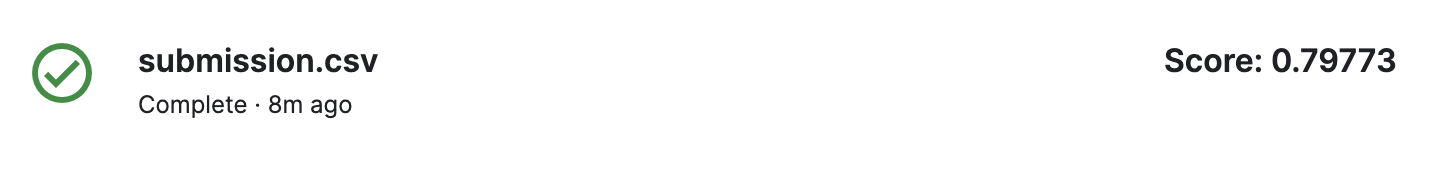
\includegraphics[width=100mm]{HW2/images/img2.png}

\end{Solution}

\section*{Written Exercises}

\setcounter{section}{0}

\section{Naive Bayes with Binary Features}
\setcounter{Problem}{0}
\begin{Problem}
    Consider a group of 80 Cornell Students. 30 of them are Master's students, while the other 50 of them are PhD students. There are 8 Master's students who bike, and there are 9 Master's students who ski. On the other hand, $30 \mathrm{PhD}$ students bike, and $12 \mathrm{PhD}$ students ski.

    We can formulate this as a machine learning problem by modeling the students with features $x=$ $\left(x_{1}, x_{2}\right) \in\{0,1\}^{2}$, where $x_{1}$ is a binary indicator of whether the students bike and $x_{2}$ is a binary indicator of whether they ski, and the target $y$ equals 1 if they are $\mathrm{PhD}$ students and 0 if they are Master's students.
\end{Problem}

\begin{Problem*}[(a)]
Please elaborate in this context what is the Naive Bayes assumption.
\end{Problem*}
\begin{Solution}
In this context, the Naive Bayes assumption is that the probability of students who bike or ski are conditionally independent given their level of education. 

$$
P\left(x \mid y\right)=P\left(x_{1} \mid y\right) \cdot P\left(x_{2} \mid y\right)\\
$$
where\\ $x_1$ is a student who bikes \newline $x_2$ is a student who skis
\end{Solution}

\begin{Problem*}[(b)]
With the Naive Bayes assumption, find the probability of a student in this group who neither bikes or skis being a Master's student
\end{Problem*}

\begin{Solution}

Let:\\
$x_{1}$ be students who bike,\\
$x_{2}$ be students who ski,\\
$y=0$ be Master's Students,\\
and $y=1$ be PhD Students

Probabilities of level of education:
\begin{align*}
    P\left(y=0\right) &= \frac{20}{50} & P\left(y=1\right) &= \frac{30}{50}\\
    &= \boxed{\frac{2}{5}} & &= \boxed{\frac{3}{5}}
\end{align*}

Probabilities of students who bike:
\begin{align*}
    P\left(x_{1}=1 \mid y=0\right) &= \frac{5}{20} & P\left(x_{1}=1 \mid y=1\right) &= \frac{20}{30}\\
    &= \boxed{\frac{1}{4}} & &= \boxed{\frac{2}{3}}
\end{align*}

Probabilities of students don't bike:
\begin{align*}
    P\left(x_{1}=0 \mid y=0\right) &= 1 - \frac{1}{4} & P\left(x_{1}=0 \mid y=1\right) &= 1 - \frac{2}{3}\\
    &= \boxed{\frac{3}{4}} & &= \boxed{\frac{1}{3}}
\end{align*}

Probabilities of students who ski:
\begin{align*}
    P\left(x_{2}=1 \mid y=0\right) &= \frac{5}{20} & P\left(x_{2}=1 \mid y=1\right) &= \frac{15}{30}\\
    &= \boxed{\frac{1}{4}} & &= \boxed{\frac{1}{2}}
\end{align*}

Probabilities of students don't ski:
\begin{align*}
    P\left(x_{2}=0 \mid y=0\right) &= 1 - \frac{1}{4} & P\left(x_{2}=0 \mid y=1\right) &= 1 - \frac{1}{2}\\
    &= \boxed{\frac{3}{4}} & &= \boxed{\frac{1}{2}}
\end{align*}

Probability of a Master's student who does not ski or bike:
\begin{align*}
    P\left(x_{1}=0, x_{2}=0\mid y=0\right) &= P\left(x_{1}=0 \mid y=0\right) \cdot P\left(x_{2}=0 \mid y=0\right)\\
    &= \frac{3}{4} \cdot \frac{3}{4}\\
    &= \boxed{\frac{9}{16}}
\end{align*}

Probability of a PhD student who does not ski or bike:
\begin{align*}
    P\left(x_{1}=0, x_{2}=0\mid y=1\right) &= P\left(x_{1}=0 \mid y=1\right) \cdot P\left(x_{2}=0 \mid y=1\right)\\
    &= \frac{1}{3} \cdot \frac{1}{2}\\
    &= \boxed{\frac{1}{6}}
\end{align*}

Probability of a student to neither ski nor bike:
\begin{align*}
    P\left(x_{1}=0, x_{2}=0\right) &= P\left(x_{1}=0, x_{2}=0\mid y=0\right) \cdot P\left(y=0\right) + P\left(x_{1}=0, x_{2}=0\mid y=1\right) \cdot P\left(y=1\right)\\
    &= \frac{9}{16} \cdot \frac{2}{5} + \frac{1}{6} \cdot \frac{3}{5}\\
    &= \boxed{\frac{13}{40}}
\end{align*}

Probability of a student in this group who neither bikes or skis being a Master’s student:
\begin{align*}
    P\left(y=0 \mid x_{1}=0, x_{2}=0\right)&=P\left(y=0\right) \cdot \frac{P\left(x_{1}=0, x_{2}=0\mid y=0\right)}{P\left(x_{1}=0, x_{2}=0\right)}\\
    &= \frac{2}{5} \cdot \frac{\frac{9}{16}}{\frac{13}{40}}\\
    &= \boxed{\frac{9}{13}}
\end{align*}

\end{Solution}

\begin{Problem*}[(c)]
Suppose we know that every $\mathrm{PhD}$ who skis also bikes. Does it make sense to still assume that probability of biking and skiing are conditionally independent for a PhD student? If not, how would your answer to part (b) change with this knowledge (you can still assume probability of biking and skiing are conditionally independent for a Master's student)?
\end{Problem*}

\begin{Solution}
    No. If we know that every PhD student who skis also bikes, then we cannot assume that the probability of biking and skiing are still conditionally independent.

    New probability of a PhD student who bikes but does not ski:
    \begin{align*}
    \begin{split}
        P\left(x_{1}=1, x_{2}=0 \mid y=1\right) &= P\left(x_{1}=1 \mid y=1\right) - P\left(x_{2}=1 \mid y=1\right)\\
        &= \frac{2}{3} - \frac{1}{2} \\
        &= \boxed{\frac{1}{6}}
    \end{split}
    \end{align*}

    New probability of a PhD student who does not ski or bike:
\begin{align*}
    P\left(x_{1}=0, x_{2}=0\mid y=1\right) &= 1 - \left(P\left(x_{1}=0, x_{2}=0 \mid y=1\right) + P\left(x_{1}=1, x_{2}=0 \mid y=1\right) + P\left(x_{1}=0, x_{2}=1 \mid y=1\right)\right) \\
    &= 1 - \left(\frac{1}{2} + \frac{1}{6} + 0 \right) = 1 - \frac{2}{3} \\
    &= \boxed{\frac{1}{3}}
\end{align*}

    New probability of a student to neither ski nor bike:
\begin{align*}
\begin{split}
     P\left(x_{1}=0, x_{2}=0\right) &= P\left(x_{1}=0, x_{2}=0\mid y=0\right) \cdot P\left(y=0\right) + P\left(x_{1}=0, x_{2}=0\mid y=1\right) \cdot P\left(y=1\right)\\
    &= \frac{9}{16} \cdot \frac{2}{5} + \frac{1}{3} \cdot \frac{3}{5}\\
    &= \boxed{\frac{17}{40}}
\end{split}
\end{align*}

    New probability of a student in this group who neither bikes or skis being a Master’s student:
\begin{align*}
    P\left(y=0 \mid x_{1}=0, x_{2}=0\right)&=P\left(y=0\right) \cdot \frac{P\left(x_{1}=0, x_{2}=0\mid y=0\right)}{P\left(x_{1}=0, x_{2}=0\right)}\\
    &= \frac{2}{5} \cdot \frac{\frac{9}{16}}{\frac{17}{40}}\\
    &= \boxed{\frac{9}{17}}
\end{align*}

\end{Solution}
\section{Categorical Naive Bayes}

\begin{Problem*}
Suppose we are working with a dataset $\mathscr{D}=\left\{\left(x^{(i)}, y^{(i)}\right) \mid y=1,2, \ldots, n\right\}$ in which the $d$-dimensional inputs $x$ are categorical: each feature $x_{j}$ takes one of $L$ possible values: $x_{j}^{(i)} \in\{1,2, \ldots, L\}$ for all $i, j$. If $L=2$, then the features look like the binary bag-of-words vectors that we have seen in class; in this example, however, the features can take more than just two values. We also assume that the target $y$ represents one of $K$ possible classes: $y \in\{1,2, \ldots, K\}$

In the Categorical Naive Bayes algorithm, we model this data via a probabilistic model $P_{\theta}(x, y)$.

\begin{itemize}
  \item The distribution $P_{\theta}(y)$ is Categorical with parameters $\phi=\left(\phi_{1}, \ldots, \phi_{K}\right)$ and
\end{itemize}

$$
P_{\theta}(y=k)=\phi_{k}
$$

\begin{itemize}
  \item The distribution of each feature $x_{j}$ conditioned on $y=k$ is a Categorical distribution with parameters $\psi_{j k}=\left(\psi_{j k 1}, \ldots, \psi_{j k L}\right)$, where
\end{itemize}

$$
P_{\theta}\left(x_{j}=\ell \mid y=k\right)=\psi_{j k \ell} .
$$

The distribution over a vector of features $x$ is given by

$$
P_{\theta}(x \mid y=k)=\prod_{j=1}^{d} P_{\theta}\left(x_{j} \mid y=k\right),
$$

which is just the Naive Bayes factorization of $P_{\theta}(x \mid y=k)$.

In other words, the prior distribution $P_{\theta}(y)$ in this model is the same as in Bernoulli Naive Bayes. The distribution $P_{\theta}(x \mid y=k)$ is a product of Categorical distributions, whereas in Bernoulli Naive Bayes it was the product of Bernoulli distributions.

The total set of parameters of this model is $\theta=\left(\phi_{1}, \ldots \phi_{K}, \psi_{111}, \ldots \psi_{d K L}\right)$. We learn the parameters via maximum likelihood:

$$
\max _{\theta} \frac{1}{n} \sum_{i=1}^{n} \log P_{\theta}\left(x^{(i)}, y^{(i)}\right)
$$
\end{Problem*} 

\begin{Problem*}[(a)]
    Show that the maximum likelihood estimate for the parameters $\phi_{k}$ is

$$
\phi_{k}^{*}=\frac{n_{k}}{n},
$$

where $n_{k}$ is the number of data points with class $k$.
\end{Problem*}

\begin{Solution}
\begin{align*}
    P_{\theta}(y)&=\phi_{k}\\
    P_{\theta}(x \mid y)&=\psi_{jk \ell}\\
    P_{\theta}(x \mid y=k)&=\prod_{j=1}^{d} P_{\theta}\left(x_{j} \mid y=k\right)\\
    P(x^{(i)}, y^{(i)}) &= \log P_{\theta}\left(x^{(i)}, y^{(i)}\right) \\
    &= \log \prod_{j=1}^{d} P\left(x_{j} \mid y=k\right)
\end{align*}

Bernoulli distribution,
\begin{equation*}
     P\left(x \right)&= p^{x}(1 - p)^{1-x}
\end{equation*}

\begin{align*}
    P\left(x_{j} \mid y=k\right)&=P\left( x_{j}, \phi_{k} \right)\\
    &= \phi_{k}^{x_{j}}\left(1 - \phi_{k} \right)^{1-x_{j}} \\
    \prod_{j=1}^{d} P\left( x_{j}, \phi_{k} \right) &= \prod_{j=1}^{d} \phi_{k}^{x_{j}}\left(1 - \phi_{k} \right)^{1-x_{j}} \\
    \log \prod_{j=1}^{d} \phi_{k}^{x_{j}}\left(1 - \phi_{k} \right)^{1-x_{j}} &= \sum_{j=1}^{n} \log\phi_{k}^{x_{j}} + \sum_{j=1}^{n} \log\left(1 - \phi_{k} \right)^{1-x_{j}}\\
    &= \sum_{j=1}^{n} x_{j}\log\phi_{k} + \sum_{j=1}^{n} (1-x_{j})\log\left(1 - \phi_{k} \right)\\
    &= \log\phi_{k} \sum_{j=1}^{n} x_{j} + \log\left(1 - \phi_{k} \right) \sum_{j=1}^{n} (1-x_{j})\\
    &= \log\phi_{k} \sum_{j=1}^{n} x_{j} + \log\left(1 - \phi_{k} \right)\left(n - \sum_{j=1}^{n} x_{j} \right) \\
\end{align*}

Setting the derivative = 0
\begin{align*}
    0 &= \frac{\sum_{j=1}^{n} x_{j}}{\phi_{k}^{*}} - \frac{n - \sum_{j=1}^{n} x_{j}}{\left( 1 -\phi_{k}^{*}\right)}\\
    &= \frac{\left( 1 -\phi_{k}^{*}\right)\sum_{j=1}^{n} x_{j} - \phi_{k}^{*}n - \sum_{j=1}^{n} x_{j}}{\phi_{k}^{*}\left( 1 -\phi_{k}^{*}\right)}\\
    &= \left( 1 -\phi_{k}^{*}\right)\sum_{j=1}^{n} x_{j} - \phi_{k}^{*}n - \sum_{j=1}^{n} x_{j}\\
    &= \sum_{j=1}^{n} x_{j} - \cancel{\phi_{k}^{*}\sum_{j=1}^{n} x_{j}} - n\phi_{k}^{*} + \cancel{\phi_{k}^{*}\sum_{j=1}^{n} x_{j}}\\
    &= \sum_{j=1}^{n} x_{j} - n\phi_{k}^{*} \\
    &= \boxed{\phi_{k}^{*} = \frac{n_{k}}{n}}
\end{align*}

\end{Solution}

\begin{Problem*}[(b)]
Show that the maximum likelihood estimate for the parameters $\psi_{j k \ell}$ is

$$
\psi_{j k \ell}^{*}=\frac{n_{j k \ell}}{n_{k}}
$$

where $n_{j k \ell}$ is the number of data points with class $k$ for which the $j$-th feature equals $\ell$.
\end{Problem*}

\begin{Solution}
\begin{align*}
    \sum_{i=y^{(i)}=k} \log P\left( x_{j}^{(i)} \mid y^{(i), \psi_{j k \ell}} \right) &= \sum_{i=y^{(i)}=k} \log \left( \frac{\psi_{j k \ell}}{\sum_{k=1}^{k}\psi_{j k \ell}} \right)\\
    &= \sum_{k=1}^{k} \sum_{i=y^{(i)}=k} \log \psi_{j k \ell} - n\log \sum_{k=1}^{k}\psi_{j k \ell}
\end{align*}

Setting the derivative = 0
\begin{align*}
    \boxed{\psi_{jk\ell}^{*} = \frac{n_{jk \ell}}{n_{k}}}
\end{align*}
\end{Solution}

%%%%%%%%%%%%%%%%%%%%%%%%%%%%%%%%%%%%%%%%%%%%%%%%%%%%%%%%%%%%%%%%%%
%Complete the assignment now
\end{document}

%%%%%%%%%%%%%%%%%%%%%%%%%%%%%%%%%%%%%%%%%%%%%%%%%%%%%%%%%%%%%%%%%%
%%%%%%%%%%%%%%%%%%%%%%%%%%%%%%%%%%%%%%%%%%%%%%%%%%%%%%%%%%%%%%%%%%
